\chapter{Problemstellung}

\section{Beschreibung}

Im Teilprojekt B3 des Sonderforschungsbereichs Transregio 62 werden aktuell Regeln zur Bewertung der Ausgabegeräte verwendet.
Dies läuft im Moment wie folgt ab:
\begin{figure}[ht]
    \centering
    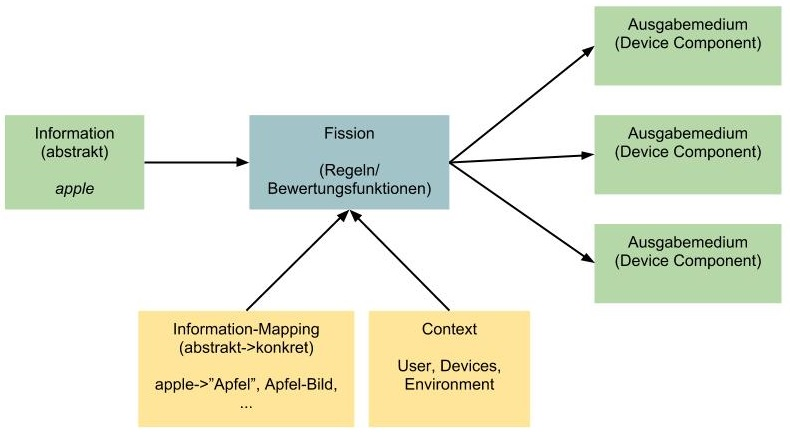
\includegraphics[width=.8\textwidth]{images/FissionUebersicht}
    \caption{\label{fission}Vereinfachte Übersicht der Funktionsweise der Fission}
\end{figure}

 Abstrakte Informationen werden vom Dialog-Manager an die Fission gesendet. Diese abstrakten Informationen werden dann von der Fission wie in Abbildung \ref{fission} zu sehen verarbeitet. Die Fission legt mittels eines Information-Mappings fest, wie die abstrakten Informationen als konkrete Informationen dargestellt werden können. So könnte zum Beispiel die abstrakte Information \emph{apple} sowohl als Text als auch als Bild dargestellt werden. Diese konkreten Daten werden dann im Bezug auf die vorhandenen Kontextinformationen (wie  User-, Environment- oder Device-Context bewertet.
Die Bewertung basiert auf unterschiedlichen Bewertungsfunktionen. Eine Funktion repräsentiert dabei eine gestalterisch bewertete Aussage, z.\,B.: \glqq Es ist sehr gut den akustischen Kanal einzusetzen wenn der Nutzer blind ist.\grqq \ Außerdem besitzt jede Regel einen Funktionswert, der positiv oder negativ sein kann. Alle Regeln werden dann auf alle Kombinationen aus konkreten Informationen und Ausgabemedien(Devices) angewendet. Dabei kann jede Regel mit einer unterschiedlichen Gewichtung in die Bewertung einfließen. Die Gewichtung geht aus dem Kontext hervor.
\linebreak
Dieser Ansatz der Bewertung hat vermutlich exponentielle Laufzeitkomplexität. Davon ausgehend, dass bereits ein weitestgehend optimaler Algorithmus genutzt wird um die Bewertung der Regeln zu berechnen soll dieser Ansatz nun evaluiert werden. Dies dient dazu Aussagen über den Einfluss der Variablen auf die Laufzeit treffen zu können. 
